\documentclass[11pt]{article}

\usepackage{amsmath}
\usepackage{minted}
\usepackage{hyperref}
\usepackage[margin=2.0cm]{geometry}

\usepackage{graphicx}
\graphicspath{ {/home/ubuntu/www/octopress/source/} }

\def\title{Singular Value Decomposition}
\newcommand\del[1]{\left(#1\right)}
\newcommand\nicefrac[2]{\frac{#1}{#2}}
\newcommand\set[1]{\left\{#1\right\}}
\newcommand\cF{\mathcal{F}}
\newcommand\Asterisk{*}

\setlength\parindent{1cm}

\begin{document}

One of the most beautiful and useful results from linear algebra, in my opinion, is a matrix
decomposition known as the \textbf{singular value decomposition}. I'd like to go over the theory
behind this matrix decomposition and show you a few examples as to why it's one of the most useful
mathematical tools you can have.

\subsection*{Diagonalization}

Before getting into the singular value decomposition (SVD), let's quickly go over diagonalization. A
matrix $A$ is \textbf{diagonalizable} if we can rewrite it (decompose it) as a product
\[A = PDP^{-1},\]
where $P$ is an invertible matrix (and thus $P^{-1}$ exists) and $D$ is a diagonal matrix (where all
off-diagonal elements are zero).

Just from this definition, we can deduce a few important things about diagonalization. First of all,
since $P$ is invertible, it must be square; therefore, this definition really only makes sense for
square matrices. A matrix that isn't square is not diagonalizable, simply because the concept of
diagonalization makes no \emph{sense} for non-square matrices. 

Another useful note is that if $A = PDP^{-1}$, then $AP = PD$.
Let's define $P$ through its columns $a_i$ and $D$ via its diagonal entries, as such:
\begin{align*}
    P &= \del{\begin{matrix}a_1 & a_2 & \dots & a_n\end{matrix}} \\
    D &= \begin{bmatrix}
        \lambda_1   & 0         & \cdots & 0 \\
        0           & \lambda_2 & \cdots & 0 \\
        \vdots      & \cdots    & \ddots & \vdots \\
        0           & \cdots    & 0      & \lambda_n
    \end{bmatrix}
\end{align*}
Due to the way matirix multiplication works, each non-zero element in $D$ (on the diagonal) simply
picks out a different column in $P$ and scales it. Namely, if we do the matrix multiplication, we
find that 
\[PD = \del{\begin{matrix}\lambda_1 a_1 & \lambda_2 a_2 & \dots & \lambda_n a_n\end{matrix}}\]

What we can draw from this is that since $AP = PD$, and we can consider the columns of $P$
separately from each other, the columns of $P$ must be the eigenvectors of $A$ and the values on the
diagonal must be eigenvalues of $A$. (Since $P$ is invertible, the space spanned by the eigenvectors
must be the entire vector space, so the eigenvectors actually form a basis. Not all matrices are
diagonalizable, since clearly not all matrices have eigenvectors that form a basis!)

In some sense, the singular value decomposition is essentially diagonalization in a more general
sense. The singular value decomposition plays a similar role to diagonalization, but it fixes the
flaws we just talked about; namely, the SVD applies to matrices of \emph{any} shape. Not only that,
but the SVD applies to \emph{all} matrices, which makes it much more generally applicable and useful
than diagonalization!

\subsection*{Singular Value Decomposition}

To get the singular value decomposition, we can take advantage of the fact that for any matrix $A$,
$A^TA$ is symmetric (since $(A^TA)^T = A^T(A^T)^T = A^TA$). Symmetric matrices have the nice
property that their eigenvectors form an orthonormal basis; this isn't terribly hard to prove, but
for the sake of brevity, take my word for it. (To prove part of this theorem, start with two
eigenvectors $v_1$ and $v_2$, write their dot product as a matrix multiplication, and essentially
fiddle with the algebra and their eigenvalues $\lambda_1$ and $\lambda_2$ until you can show that
the dot product must be zero because the eigenvalues are distinct.)

Since symmetric matrices have an orthonormal basis of eigenvectors, consider the eigenvectors $x_i$
and corresponding eigenvalues $\lambda_i$. Let $\sigma_i = \sqrt{\lambda_i}$, and let 
$r_i = \frac{A x_i}{\sigma_i}$. Let's construct three matrices from these values: the diagonal
matrix $\Sigma$, which has  $\sigma_i$ values on the diagonal (padded with zeros if we run out of
$\sigma$s); the matrix $U$ with $r_i$s as columns; and the matrix $V$ with $x_i$s as the columns. 
(As an example, consider an $A$ that is 500x800; then, $U$ will be 500x500, $\Sigma$ will be
500x800, with the rightmost 300 columns being just zeros, and $V$ will be 800x800.)

Let's look at $U\Sigma V^T$, and perform this multiplication step-by-step. First, start by computing
$U\Sigma$; like before, the diagonal entries in $\Sigma$ scale the columns of $U$, so we get a
matrix with columns that look like 
\[\sigma_i r_i = \sigma_i \frac{A x_i}{\sigma_i} = A x_i.\] 
Next, we multiply $U\Sigma$ by $V^T$, which means we're multiplying columns that look like $Ax_i$ by
rows of the form $x_j$; note that these are \emph{rows}, since $V$ has these as columns, and we're
multiplying by $V^T$. The product contains terms that look like $Ax_i {x_j}^T$; however, since the
$x_i$s and $x_j$s are the eigenvectors of a symmetric matrix, they form an orthonormal basis! This
means that any distinct eigenvectors are orthogonal, so if $i \ne j$, $x_i {x_j}^T = 0$; since
they're \emph{ortho}normal, that means that $x_i {x_i}^T = 1$! In other words, distinct eigenvector
dot products cancel out (due to orthogonality) and non-distinct eigenvectors simply leave the matrix
$A$ alone, because their dot product is one. These $x_i {x_j}^T$ product terms form the identity
matrix, where we have ones on the diagonal (where $i = j$) and zeros elsewhere ($i \ne j$), which
yields that $U\Sigma V^T = AI = A$. Thus, we've derived the singular value decomposition in its most
common form: for any matrix $A$, we can rewrite it as the product $A = U\Sigma V^T$ of three
matrices, $U$, $\Sigma$, and $V^T$, where $U$ and $V$ have orthonormal columns and $\Sigma$ is a
diagonal matrix (the entries of which are known as \textbf{singular values}).

Though this may seem esoteric, the meaning of this theorem is fundamental and very interesting. You
can try to visualize it by considering what happens to the unit sphere in your vector space as it's
being transformed by the matrix $A$. First, we apply some transformation $V^T$, which is essentially
a rotation, since it's a matrix with orthonormal rows. (A matrix with orthonormal rows just
changes the coordinate axes via some rotation or reflection but does no scaling.) Next, we apply a
scaling defined by $\Sigma$, which just scales the dimensions since it's a diagonal matrix. Finally,
we rotate again with $U$, and we're done! In other words, any transformation can be expressed as a
rotation followed by a scaling followed by another rotation. And that's pretty cool! Not only is it
cool - it's also thoroughly useful all over mathematics and computer science.\\

\noindent \emph{\textbf{Note:} this interpretation is specific for real square matrices, and that as soon as you start
dealing with complex-valued matrices or non-square matrices this geometric interpretation loses its
meaning.}

\subsection*{Applications: Data Compression}

The SVD is a thoroughly useful decomposition, useful for a whole \emph{ton} of stuff. I'd like to
quickly provide you with some examples, just to show you a small glimpse of what this can be used
for in computer science, math, and other disciplines.

One application of the SVD is data compression. Consider some matrix $A$ with rank five hundred; that
is, the columns of this matrix span a 500-dimensional space. Encoding this matrix on a computer is going to take
quite a lot of memory! We might be interested in \emph{approximating} this matrix with one of
lower rank - how close can we get to this matrix if we only approximate it as a matrix with rank one
hundred, so that we only have to store a hundred columns? What if we use a matrix of rank twenty?
Can we summarize all of the information in this very dense, 500-rank matrix with only a rank twenty
matrix?

It turns out that you can prove that taking the $n$ largest singular values $A$, replacing the rest with
zero (to form $\Sigma'$), and recomputing $U\Sigma' V^T$ gives you the provably-best $n$-rank
approximation to the matrix. Not only that, but the total of the first $n$ singular values divided
by the sum of all the singular values is the percentage of ``information'' that those singular
values contain. If we want to keep 90\% of the information, we just need to compute sums of singular
values until we reach 90\% of the sum, and discard the rest of the singular values. This yields a
quick and dirty compression algorithm for matrices - take the SVD, drop all but a few singular
values, and then recompute the approximated matrix. Since we only need to store the columns of $U$
and $V$ that actually get used (many get dropped since we set elements on the diagonal of $\Sigma$
to zero), we greatly reduce the memory usage.\\

\noindent Here's a tiger:\\

\includegraphics[scale=0.3]{images/tiger.jpg}\\

We can convert this tiger to black and white, and then just treat this tiger as a matrix, where each
element is the pixel intensity at the relevant location. Here are the singular values of this tiger:\\
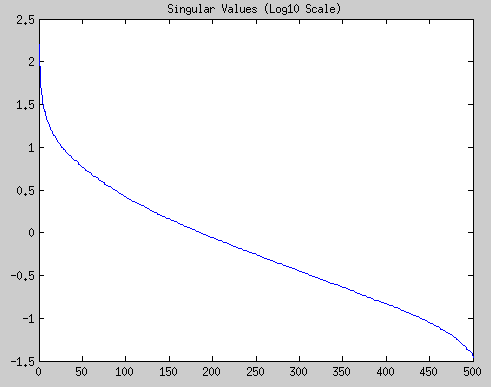
\includegraphics[scale=0.5]{images/singular_values.png}\\

Note that this is a log scale (base 10). Most of the action and the largest singular values are the
first thirty or so, and they contain a majority of the ``information'' in this matrix! We can plot
the cumulative percentage, to see how much the first thirty or fifty singular values contain of the
information:\\
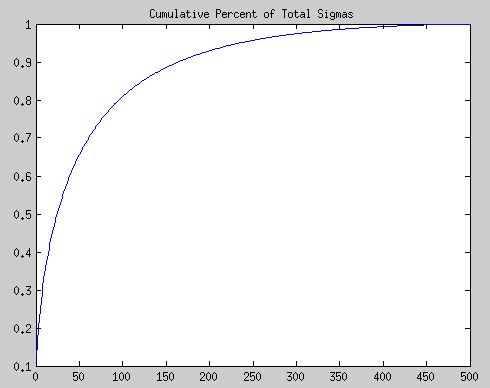
\includegraphics[scale=0.5]{images/sigmas_cumsum.png}\\

After just fifty of the singular values, we already have over 70\% of the information contained in
this tiger! Finally, let's take some approximations and plot a few approximate tigers:\\
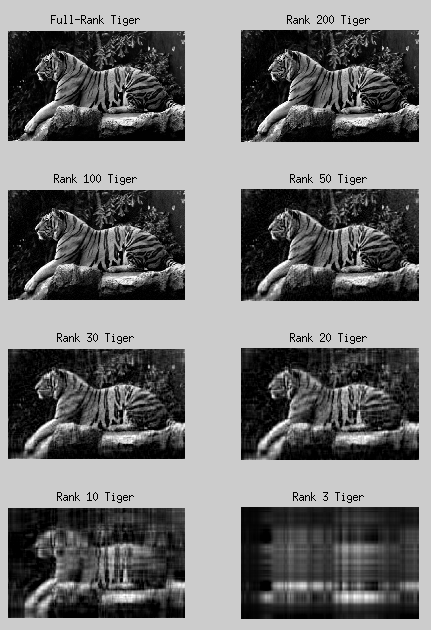
\includegraphics[scale=0.6]{images/tigers.png}\\

Note that after about thirty or fifty components, adding more singular values doesn't visually seem
to improve image quality. By a quick application of SVD, you've just compressed a 500x800 pixel
image into a 50x500 matrix (for $U$), 50 singular values, and a 800x50 matrix (for $V$). The MATLAB
code for generating these is incredibly straight-forward, as follows below.\\

\textbf{Low-Rank Matrix Approximation Image Compression} \href{http://andrew.gibiansky.com/downloads/code/compress.m}{(download)}
\begin{minted}{matlab}
% Read the picture of the tiger, and convert to black and white.
tiger = rgb2gray(imread('tiger.jpg'));

% Downsample, just to avoid dealing with high-res images.
tiger = im2double(imresize(tiger, 0.5));

% Compute SVD of this tiger
[U, S, V] = svd(tiger);

% Plot the magnitude of the singular values (log scale)
sigmas = diag(S);
figure; plot(log10(sigmas)); title('Singular Values (Log10 Scale)');
figure; plot(cumsum(sigmas) / sum(sigmas)); title('Cumulative Percent of Total Sigmas');

% Show full-rank tiger
figure; subplot(4, 2, 1), imshow(tiger), title('Full-Rank Tiger');

% Compute low-rank approximations of the tiger, and show them
ranks = [200, 100, 50, 30, 20, 10, 3];
for i = 1:length(ranks)
    % Keep largest singular values, and nullify others.
    approx_sigmas = sigmas; approx_sigmas(ranks(i):end) = 0;

    % Form the singular value matrix, padded as necessary
    ns = length(sigmas);
    approx_S = S; approx_S(1:ns, 1:ns) = diag(approx_sigmas);

    % Compute low-rank approximation by multiplying out component matrices.
    approx_tiger = U * approx_S * V';

    % Plot approximation
    subplot(4, 2, i + 1), imshow(approx_tiger), title(sprintf('Rank %d Tiger', ranks(i)));
end
\end{minted}

\subsection*{Applications: Solving Linear Equations}

Another common application of the singular value decomposition is in fitting solutions to linear
equations. Suppose we collect a ton of data, which we believe can be fit to some linear homogeneous
equation. If we have our data in a matrix $A$, and our variables in some vector $x$, we can write
this problem as $Ax = 0$, where we'd like to figure out what $x$ is given $A$. Of course, we may
have more data than variables (in fact, we \emph{should}!), in which case we can't \emph{solve}
this; however, we can fit $x$ to $A$ in order to minimize the value of $Ax$. It turns out that you
can do this via a singular value decomposition!

Let's start form the beginning. For the sake of demonstration, suppose you have a ton of points that
look like this:\\
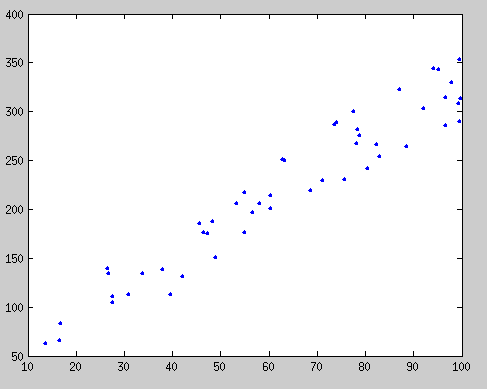
\includegraphics[scale=0.5]{images/random_points.png}\\

Each point is an $(x_i, y_i)$ pair. We hypothesize that these are related by the linear equation
$ax_i + by_i = c$, since the relationship looks pretty linear in that graph. Equivalently, $ax_i +
by_i - c = 0$, or, in vector form (combining all equations into one), 
\[a\begin{bmatrix}x_1 \\ x_2 \\ \vdots \\ x_n\end{bmatrix} + b\begin{bmatrix}y_1 \\ y_2 \\ \vdots \\
y_n\end{bmatrix} + c\begin{bmatrix}-1 \\ -1 \\ \vdots \\ -1\end{bmatrix} = \begin{bmatrix}
x_1 & y_1 & -1 \\ x_2 & y_2 & -1 \\ \vdots & \vdots & \vdots \\ x_n & y_n & -1 \\
\end{bmatrix}\begin{bmatrix}a \\ b \\ c\end{bmatrix} = \textbf{0}.\]

Since we can't solve this exactly, we'd really like to minimize that value, even if we can't set it
to \textbf{0}. However, note that by setting $a$, $b$, and $c$ arbitrarily small, we can get that
value as small as we want to, so to combat this we force a scale by requiring that the vector
$\begin{bmatrix}a & b & c\end{bmatrix}$ be unit normal (namely, $\sqrt{a^2 + b^2 + c^2} = 1$). This
is the general problem of linear data fitting, and this type of scale-normalization is always
required for homogeneous equation fitting.

Let's consider our data matrix, 
\[A = \begin{bmatrix}
        x_1 & y_1 & -1 \\ x_2 & y_2 & -1 \\ \vdots & \vdots & \vdots \\ x_n & y_n & -1 \\
\end{bmatrix}.\]
Suppose we take the singular value decomposition of $A$ to get $A = U\Sigma V^T$. If the equation
$Ax=0$ can be solved exactly, then at least one of the eigenvalues of $A$ must be zero, which in
turn means that one of the eigenvalues of $AA^T$ must be zero, and therefore one of the singular
values must be zero. So, if one of elements on the diagonal of $\Sigma$ is zero, then we have a
solution! In fact, that solution corresponds to the column of $V$ that corresponds to the
zero-valued singular value. We can look for a zero-valued singular value, take the corresponding
column of $V$, and have our linear solution! (Note that if we have two zero
singular values, that just means that we have multiple solutions to our
equation, and the system of equations is underconstrained.  Though the
solutions are not going to be orthogonal, they can still be linearly
independent and span a multidimensiional solution space.)

If none of the singular values are zero, we have no solution to our equation. Although it's slightly
tricky to prove, I think you'll find it very intuitive that the \emph{smallest} singular value
actually corresponds to the solution to the linear least squares fitting problem! Namely, if you
want to find the least squares fit to the data, simply look at the smallest (usually, last) singular
value, take the corresponding column of $V$, and read off your covariate values. In this case, we
can compute the singular value decomposition of $A$, and then look at the third column of $V$ and
read off the values of $a$, $b$, and $c$, directly from that column of $V$. The resulting fit looks
like this:\\
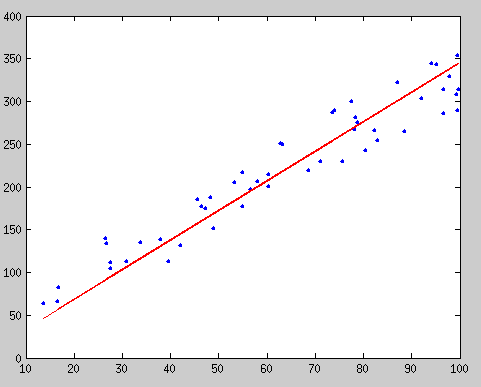
\includegraphics[scale=0.6]{images/random_points_fit.png}\\

The MATLAB code for generating the points and doing the fit is below.

\textbf{Homogenous Linear Equation Fitting} \href{http://andrew.gibiansky.com/downloads/code/points.m}{(download)}
\begin{minted}{matlab}
% Generate some points around a line
intercept = -10; slope = 3;
npts = 50; noise = 80;
xs = 10 + rand(npts, 1) * 90;
ys = slope * xs + intercept + rand(npts, 1) * noise;

% Plot the randomly generated points
figure; plot(xs, ys, 'b.', 'MarkerSize', 5)

% Fit these points to a line
A = [xs, ys, -1 * ones(npts, 1)];
[U, S, V] = svd(A);
fit = V(:, end - 1);

% Get the coefficients a, b, c in ax + by + c = 0
a = fit(1); b = fit(2); c = fit(3);

% Compute slope m and intercept i for y = mx + i
slope_est = -a / b;
intercept_est = c / b;

% Plot fitted line on top of old data
ys_est = slope_est * xs + intercept_est;
figure; plot(xs, ys, 'b.', 'MarkerSize', 5);
hold on; plot(xs, ys_est, 'r-')
\end{minted}

\subsection*{Summary}
The singular value decomposition (SVD) is an incredibly useful tool, and you'll find it scattered
throughout almost very scientific discipline. For instance, it can be used for efficiently
simulating high-dimensional partial differential equations by taking all the data generated from the
simulations, reducing the data dimensionality by throwing away some of the singular values, and then
simulating the lower-dimensional system. The fact that SVD gives us an optimal low-rank
representation guarantees that this sort of simulation preserves most of the detail in a system, as
getting rid of the extra modes (singular values) in the system is guaranteed to get rid of the least
important modes. In a slightly different vein, the SVD is used everywhere from physics to machine
learning for dimensionality reduction; the algorithm commonly known as Principal Component Analysis
(PCA), for instance, is just a simple application of the singular value decomposition. In computer
vision, the first face recognition algorithms (developed in the 1970's and 1980's) used PCA and SVD
in order to represent faces as a linear combination of ``eigenfaces'', do dimensionality
reduction, and then match faces to identities via simpler methods; although modern methods are much
more sophisticated, many still depend on similar techniques.

In summary, if there's anything at all you remember and treasure from linear algebra, it should be
the singular value decomposition. It's \emph{everywhere}.

\end{document}
